

\tikzset{every picture/.style={line width=0.75pt}} %set default line width to 0.75pt        

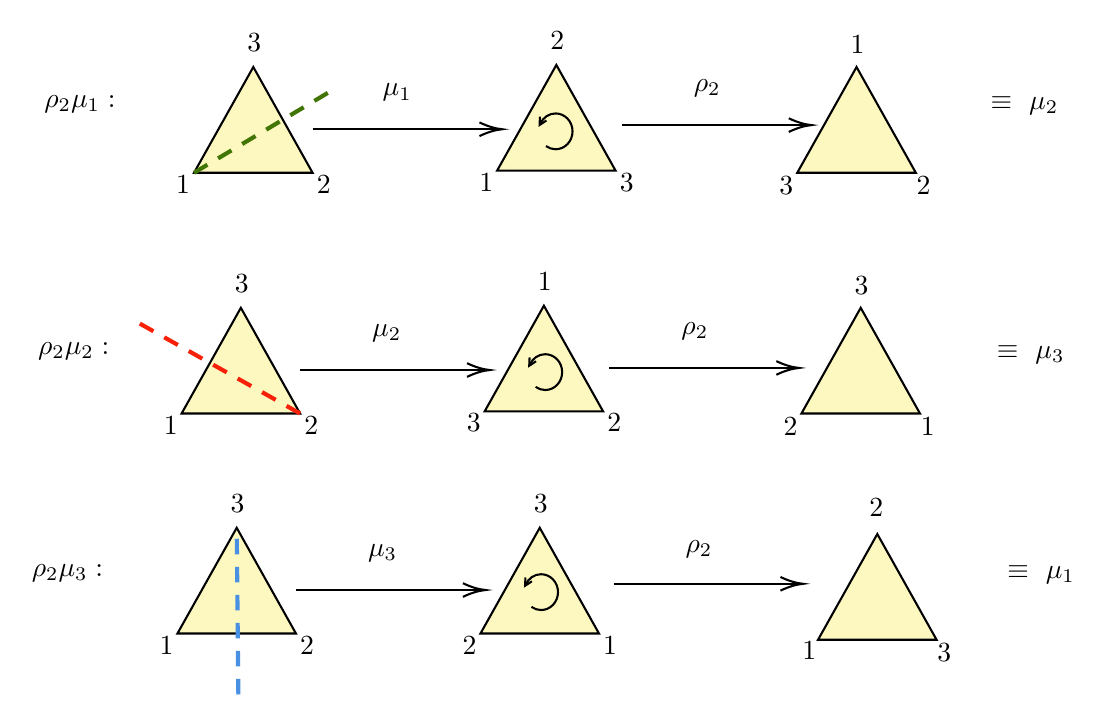
\begin{tikzpicture}[x=0.75pt,y=0.75pt,yscale=-1,xscale=1]
%uncomment if require: \path (0,341); %set diagram left start at 0, and has height of 341

%Shape: Triangle [id:dp38083149863639465] 
\draw  [fill={rgb, 255:red, 250; green, 238; blue, 106 }  ,fill opacity=0.43 ] (298.21,252.26) -- (326.76,303.2) -- (269.65,303.2) -- cycle ;

%Shape: Triangle [id:dp8834642070216787] 
\draw  [fill={rgb, 255:red, 250; green, 238; blue, 106 }  ,fill opacity=0.43 ] (300.21,145.26) -- (328.76,196.2) -- (271.65,196.2) -- cycle ;

%Shape: Triangle [id:dp8480067615213543] 
\draw  [fill={rgb, 255:red, 250; green, 238; blue, 106 }  ,fill opacity=0.43 ] (306.21,29.26) -- (334.76,80.2) -- (277.65,80.2) -- cycle ;

%Shape: Triangle [id:dp3963964289598798] 
\draw  [fill={rgb, 255:red, 250; green, 238; blue, 106 }  ,fill opacity=0.43 ] (452.85,146.26) -- (481.41,197.2) -- (424.29,197.2) -- cycle ;
%Shape: Triangle [id:dp7042235181906016] 
\draw  [fill={rgb, 255:red, 250; green, 238; blue, 106 }  ,fill opacity=0.43 ] (154.21,146.26) -- (182.76,197.2) -- (125.65,197.2) -- cycle ;

%Straight Lines [id:da513809238677429] 
\draw    (331.75,175.24) -- (421.12,175.24) ;
\draw [shift={(423.12,175.24)}, rotate = 180] [color={rgb, 255:red, 0; green, 0; blue, 0 }  ][line width=0.75]    (10.93,-3.29) .. controls (6.95,-1.4) and (3.31,-0.3) .. (0,0) .. controls (3.31,0.3) and (6.95,1.4) .. (10.93,3.29)   ;
%Shape: Arc [id:dp0752155899104685] 
\draw  [draw opacity=0] (293.49,173.52) .. controls (294.81,170.63) and (297.61,168.62) .. (300.85,168.62) .. controls (305.36,168.62) and (309.01,172.49) .. (309.01,177.25) .. controls (309.01,182.02) and (305.36,185.88) .. (300.85,185.88) .. controls (299.13,185.88) and (297.53,185.31) .. (296.21,184.35) -- (300.85,177.25) -- cycle ; \draw   (293.49,173.52) .. controls (294.81,170.63) and (297.61,168.62) .. (300.85,168.62) .. controls (305.36,168.62) and (309.01,172.49) .. (309.01,177.25) .. controls (309.01,182.02) and (305.36,185.88) .. (300.85,185.88) .. controls (299.13,185.88) and (297.53,185.31) .. (296.21,184.35) ;  
\draw   (296.43,172.03) -- (293.15,174.18) -- (293.31,170.2) ;

%Straight Lines [id:da014113470336568845] 
\draw [color={rgb, 255:red, 247; green, 33; blue, 9 }  ,draw opacity=1 ][line width=1.5]  [dash pattern={on 5.63pt off 4.5pt}]  (182.76,197.2) -- (105,153.58) ;
%Straight Lines [id:da4766267282251375] 
\draw    (182.75,176.24) -- (272.12,176.24) ;
\draw [shift={(274.12,176.24)}, rotate = 180] [color={rgb, 255:red, 0; green, 0; blue, 0 }  ][line width=0.75]    (10.93,-3.29) .. controls (6.95,-1.4) and (3.31,-0.3) .. (0,0) .. controls (3.31,0.3) and (6.95,1.4) .. (10.93,3.29)   ;
%Shape: Triangle [id:dp09853355186084745] 
\draw  [fill={rgb, 255:red, 250; green, 238; blue, 106 }  ,fill opacity=0.43 ] (450.85,30.26) -- (479.41,81.2) -- (422.29,81.2) -- cycle ;
%Shape: Triangle [id:dp024455387058983202] 
\draw  [fill={rgb, 255:red, 250; green, 238; blue, 106 }  ,fill opacity=0.43 ] (160.21,30.26) -- (188.76,81.2) -- (131.65,81.2) -- cycle ;

%Straight Lines [id:da4475565080931384] 
\draw    (337.75,58.24) -- (427.12,58.24) ;
\draw [shift={(429.12,58.24)}, rotate = 180] [color={rgb, 255:red, 0; green, 0; blue, 0 }  ][line width=0.75]    (10.93,-3.29) .. controls (6.95,-1.4) and (3.31,-0.3) .. (0,0) .. controls (3.31,0.3) and (6.95,1.4) .. (10.93,3.29)   ;
%Shape: Arc [id:dp7787418801052134] 
\draw  [draw opacity=0] (298.49,57.52) .. controls (299.81,54.63) and (302.61,52.62) .. (305.85,52.62) .. controls (310.36,52.62) and (314.01,56.49) .. (314.01,61.25) .. controls (314.01,66.02) and (310.36,69.88) .. (305.85,69.88) .. controls (304.13,69.88) and (302.53,69.31) .. (301.21,68.35) -- (305.85,61.25) -- cycle ; \draw   (298.49,57.52) .. controls (299.81,54.63) and (302.61,52.62) .. (305.85,52.62) .. controls (310.36,52.62) and (314.01,56.49) .. (314.01,61.25) .. controls (314.01,66.02) and (310.36,69.88) .. (305.85,69.88) .. controls (304.13,69.88) and (302.53,69.31) .. (301.21,68.35) ;  
\draw   (301.43,56.03) -- (298.15,58.18) -- (298.31,54.2) ;

%Straight Lines [id:da9005403767384724] 
\draw    (188.75,60.24) -- (278.12,60.24) ;
\draw [shift={(280.12,60.24)}, rotate = 180] [color={rgb, 255:red, 0; green, 0; blue, 0 }  ][line width=0.75]    (10.93,-3.29) .. controls (6.95,-1.4) and (3.31,-0.3) .. (0,0) .. controls (3.31,0.3) and (6.95,1.4) .. (10.93,3.29)   ;
%Straight Lines [id:da524115019147908] 
\draw [color={rgb, 255:red, 65; green, 117; blue, 5 }  ,draw opacity=1 ][line width=1.5]  [dash pattern={on 5.63pt off 4.5pt}]  (131.65,81.2) -- (198,41.58) ;
%Shape: Triangle [id:dp4811247244578286] 
\draw  [fill={rgb, 255:red, 250; green, 238; blue, 106 }  ,fill opacity=0.43 ] (460.85,255.26) -- (489.41,306.2) -- (432.29,306.2) -- cycle ;
%Shape: Triangle [id:dp23313243882490287] 
\draw  [fill={rgb, 255:red, 250; green, 238; blue, 106 }  ,fill opacity=0.43 ] (152.21,252.26) -- (180.76,303.2) -- (123.65,303.2) -- cycle ;

%Straight Lines [id:da1470468648823009] 
\draw    (333.75,279.24) -- (423.12,279.24) ;
\draw [shift={(425.12,279.24)}, rotate = 180] [color={rgb, 255:red, 0; green, 0; blue, 0 }  ][line width=0.75]    (10.93,-3.29) .. controls (6.95,-1.4) and (3.31,-0.3) .. (0,0) .. controls (3.31,0.3) and (6.95,1.4) .. (10.93,3.29)   ;
%Shape: Arc [id:dp34868135972523007] 
\draw  [draw opacity=0] (291.49,279.52) .. controls (292.81,276.63) and (295.61,274.62) .. (298.85,274.62) .. controls (303.36,274.62) and (307.01,278.49) .. (307.01,283.25) .. controls (307.01,288.02) and (303.36,291.88) .. (298.85,291.88) .. controls (297.13,291.88) and (295.53,291.31) .. (294.21,290.35) -- (298.85,283.25) -- cycle ; \draw   (291.49,279.52) .. controls (292.81,276.63) and (295.61,274.62) .. (298.85,274.62) .. controls (303.36,274.62) and (307.01,278.49) .. (307.01,283.25) .. controls (307.01,288.02) and (303.36,291.88) .. (298.85,291.88) .. controls (297.13,291.88) and (295.53,291.31) .. (294.21,290.35) ;  
\draw   (294.43,278.03) -- (291.15,280.18) -- (291.31,276.2) ;

%Straight Lines [id:da5341070876503803] 
\draw    (180.75,282.24) -- (270.12,282.24) ;
\draw [shift={(272.12,282.24)}, rotate = 180] [color={rgb, 255:red, 0; green, 0; blue, 0 }  ][line width=0.75]    (10.93,-3.29) .. controls (6.95,-1.4) and (3.31,-0.3) .. (0,0) .. controls (3.31,0.3) and (6.95,1.4) .. (10.93,3.29)   ;
%Straight Lines [id:da57458263235198] 
\draw [color={rgb, 255:red, 74; green, 144; blue, 226 }  ,draw opacity=1 ][line width=1.5]  [dash pattern={on 5.63pt off 4.5pt}]  (153,332.57) -- (152.21,252.26) ;

% Text Node
\draw (414.22,197.82) node [anchor=north west][inner sep=0.75pt]    {$2$};
% Text Node
\draw (480.3,197.82) node [anchor=north west][inner sep=0.75pt]    {$1$};
% Text Node
\draw (448.48,129.62) node [anchor=north west][inner sep=0.75pt]    {$3$};
% Text Node
\draw (365,151.91) node [anchor=north west][inner sep=0.75pt]    {$\rho _{2}$};
% Text Node
\draw (216,152.91) node [anchor=north west][inner sep=0.75pt]    {$\mu _{2}$};
% Text Node
\draw (522,268.91) node [anchor=north west][inner sep=0.75pt]    {$\equiv \ \mu _{1}$};
% Text Node
\draw (412.22,81.82) node [anchor=north west][inner sep=0.75pt]    {$3$};
% Text Node
\draw (478.3,81.82) node [anchor=north west][inner sep=0.75pt]    {$2$};
% Text Node
\draw (446.48,13.62) node [anchor=north west][inner sep=0.75pt]    {$1$};
% Text Node
\draw (371,34.91) node [anchor=north west][inner sep=0.75pt]    {$\rho _{2}$};
% Text Node
\draw (221,36.91) node [anchor=north west][inner sep=0.75pt]    {$\mu _{1}$};
% Text Node
\draw (517,162.91) node [anchor=north west][inner sep=0.75pt]    {$\equiv \ \mu _{3}$};
% Text Node
\draw (58,42.63) node [anchor=north west][inner sep=0.75pt]    {$\rho _{2} \mu _{1} :$};
% Text Node
\draw (55,161.63) node [anchor=north west][inner sep=0.75pt]    {$\rho _{2} \mu _{2} :$};
% Text Node
\draw (423.22,305.82) node [anchor=north west][inner sep=0.75pt]    {$1$};
% Text Node
\draw (488.3,306.82) node [anchor=north west][inner sep=0.75pt]    {$3$};
% Text Node
\draw (455.48,236.62) node [anchor=north west][inner sep=0.75pt]    {$2$};
% Text Node
\draw (367,256.91) node [anchor=north west][inner sep=0.75pt]    {$\rho _{2}$};
% Text Node
\draw (214,258.91) node [anchor=north west][inner sep=0.75pt]    {$\mu _{3}$};
% Text Node
\draw (514,42.91) node [anchor=north west][inner sep=0.75pt]    {$\equiv \ \mu _{2}$};
% Text Node
\draw (52,268.63) node [anchor=north west][inner sep=0.75pt]    {$\rho _{2} \mu _{3} :$};
% Text Node
\draw (147.84,234.8) node [anchor=north west][inner sep=0.75pt]    {$3$};
% Text Node
\draw (181.29,303) node [anchor=north west][inner sep=0.75pt]    {$2$};
% Text Node
\draw (113.57,303) node [anchor=north west][inner sep=0.75pt]    {$1$};
% Text Node
\draw (155.84,12.8) node [anchor=north west][inner sep=0.75pt]    {$3$};
% Text Node
\draw (189.29,81) node [anchor=north west][inner sep=0.75pt]    {$2$};
% Text Node
\draw (121.57,81) node [anchor=north west][inner sep=0.75pt]    {$1$};
% Text Node
\draw (149.84,128.8) node [anchor=north west][inner sep=0.75pt]    {$3$};
% Text Node
\draw (183.29,197) node [anchor=north west][inner sep=0.75pt]    {$2$};
% Text Node
\draw (115.57,197) node [anchor=north west][inner sep=0.75pt]    {$1$};
% Text Node
\draw (301.84,11.8) node [anchor=north west][inner sep=0.75pt]    {$2$};
% Text Node
\draw (335.29,80) node [anchor=north west][inner sep=0.75pt]    {$3$};
% Text Node
\draw (267.57,80) node [anchor=north west][inner sep=0.75pt]    {$1$};
% Text Node
\draw (295.84,127.8) node [anchor=north west][inner sep=0.75pt]    {$1$};
% Text Node
\draw (329.29,196) node [anchor=north west][inner sep=0.75pt]    {$2$};
% Text Node
\draw (261.57,196) node [anchor=north west][inner sep=0.75pt]    {$3$};
% Text Node
\draw (293.84,234.8) node [anchor=north west][inner sep=0.75pt]    {$3$};
% Text Node
\draw (327.29,303) node [anchor=north west][inner sep=0.75pt]    {$1$};
% Text Node
\draw (259.57,303) node [anchor=north west][inner sep=0.75pt]    {$2$};


\end{tikzpicture}
